% Self-contained editable report. Compile twice with:
% pdflatex -interaction=nonstopmode -halt-on-error CS6886_Report_Concise.tex
% No external figures, bibliography program, or custom class is required.
\documentclass[10pt,a4paper]{article}
\usepackage[T1]{fontenc}
\usepackage{lmodern,microtype}
\DisableLigatures{encoding = *, family = tt*}
\usepackage[margin=16mm,top=13mm,bottom=13mm]{geometry}
\usepackage{amsmath,amssymb,booktabs,tabularx,array,multicol}
\usepackage[table]{xcolor}
\usepackage{enumitem,titlesec,fancyhdr,lastpage,xurl}
\usepackage{tikz}
\usetikzlibrary{arrows.meta,positioning}
\usepackage{tcolorbox}
\usepackage[colorlinks=true,linkcolor=teal!65!black,citecolor=teal!65!black,urlcolor=teal!65!black]{hyperref}
\hypersetup{pdftitle={Compiler Optimizations for Attention and Functional KV Caches},pdfauthor={Nishanth Senthil Kumar}}
\definecolor{accent}{HTML}{176B70}
\definecolor{pale}{HTML}{EFF6F6}
\definecolor{ink}{HTML}{192A35}
\color{ink}
\setlength{\parindent}{0pt}
\setlength{\parskip}{3pt}
\setlength{\abovedisplayskip}{4pt}
\setlength{\belowdisplayskip}{4pt}
\setlength{\abovedisplayshortskip}{3pt}
\setlength{\belowdisplayshortskip}{3pt}
\setlength{\tabcolsep}{4pt}
\renewcommand{\arraystretch}{1.04}
\newcolumntype{Y}{>{\raggedright\arraybackslash}X}
\newcolumntype{P}[1]{>{\raggedright\arraybackslash}p{#1}}
\setlist[itemize]{leftmargin=13pt,itemsep=1.5pt,topsep=2pt,parsep=0pt}
\titleformat{\section}{\large\bfseries\color{accent}}{\thesection}{0.5em}{}
\titlespacing*{\section}{0pt}{4pt}{2pt}
\pagestyle{fancy}
\fancyhf{}
\fancyhead[L]{\footnotesize CS6886 \;|\; Attention compiler optimization}
\fancyhead[R]{\footnotesize 1 November 2026}
\fancyfoot[R]{\footnotesize\thepage\,/\,\pageref{LastPage}}
\renewcommand{\headrulewidth}{0.25pt}
\setlength{\headheight}{13pt}
\newcommand{\code}[1]{\texttt{#1}}
\newcommand{\sel}{\operatorname{select}}
\newcommand{\cat}{\operatorname{concat}}
\newcommand{\up}{\operatorname{update}}
\newcommand{\smallnote}[1]{{\footnotesize #1\par}}
\newtcolorbox{resultbox}{colback=pale,colframe=accent,boxrule=0.45pt,arc=1mm,left=5pt,right=5pt,top=3pt,bottom=3pt}
% Edit/add team members here as appropriate.
\newcommand{\projectauthors}{Nishanth Senthil Kumar (EE23B049) \quad IIT Madras}

\begin{document}
\thispagestyle{plain}
{\LARGE\bfseries Compiler Optimizations for Attention\\[2pt]and Functional KV Caches\par}
{\small CS6886: Systems Engineering for Deep Learning \hfill 1 November 2026\par}
{\small\projectauthors\par}
\vspace{2pt}
\begin{resultbox}
\textbf{Main result.} On a Tesla T4, winner-cache factoring lowers a pretrained two-candidate step's IREE latency by \textbf{26.46\% at context 2048}. Sparse synthetic cache forwarding reduces measured DRAM bytes by \textbf{99.92\%}. These are different workloads; full-model DRAM reduction is not consistent.
\end{resultbox}

\section{Problem and baseline investigation}
\begin{itemize}
\item \textbf{GQA and caching.} A KV cache stores earlier tokens' keys and values. With $H_q$ query and $H_{kv}$ KV heads, GQA shares each KV head across $g=H_q/H_{kv}$ query heads: $h_{kv}=\lfloor h_q/g\rfloor$~\cite{gqa,mqa}.
\item \textbf{Initial hypothesis.} Explicit \code{repeat\_interleave}/reshape can expand K/V tensors. A C++ rewrite improved the original default CPU case \textbf{18.47 to 9.94\,$\mu$s (1.86$\times$)}, but stronger existing IREE settings remove the tested expansion too.
\item \textbf{Deciding settings.} Ablation across head ratios and shapes established that both flags below were needed for the tested grouped cases; O3 alone was insufficient~\cite{ireesource,project}.
\end{itemize}
{\footnotesize\ttfamily
--iree-opt-generalize-matmul\\
--iree-dispatch-creation-enable-aggressive-reshape-movement\par}
\smallnote{The subsequent study targets missed functional-cache patterns.}

\section{Main transformations}
Let $C$ be an immutable history, $U$ a $t$-row update at position $p$, and $C'=\up(C,p,U)$.
\begin{equation*}
\underbrace{C'[i]}_{\text{read after update}}\quad\longrightarrow\quad
\begin{cases}U[i-p],&p\leq i<p+t,\\C[i],&\text{otherwise.}\end{cases}
\end{equation*}
\textbf{Read forwarding:} sparse/gather consumers access the base or patch directly. An unobserved updated tensor may disappear; a returned full cache still needs its required representation.
\begin{equation*}
\underbrace{\sel(c,\cat(C,a),\cat(C,b))}_{\text{select full candidate caches}}
\ \longrightarrow\ \underbrace{\cat(C,\sel(c,a,b))}_{\text{select small rows, then commit}}.
\end{equation*}
\textbf{Winner factoring:} same history/append axis, scalar Boolean $c$. The model has \textbf{60 matches} (K/V in 30 layers); ordinary decode has \textbf{zero}. Candidate attention computations remain.

\section{Prior work and implemented extensions}
{\small
\begin{tabularx}{\linewidth}{@{}P{30mm}YY@{}}
\toprule
\textbf{Transformation} & \textbf{Implementation / intended use} & \textbf{Boundary / prior work}\\
\midrule
Read/gather forwarding & Base-or-patch reads for forked sparse attention; normalize gather indices. & Established read-over-write algebra~\cite{mccarthy,arrays}; full cache observations remain.\\
Winner commit factoring & Select small rows before a common-history append / equal-region update. & Custom branching step; standard selection algebra, not complete beam/speculative decoding.\\
Update coalescing & Merge adjacent small writes before forwarding multi-token chains. & Reject gaps, overlaps or observed intermediate versions. Classical update simplification.\\
Snapshot protection & Preserve returned old caches and supported borrowed-buffer ownership. & Correctness repair; sharing/COW precedents~\cite{paged,forkkv}. Invalid outputs are excluded.\\
Projection / partial RoPE & $q(CW_K)^T=(qW_K^T)C^T$; project content separately from rotary coordinates. & MLA absorption / decoupled RoPE are prior art~\cite{deepseek,rope}; require a numerical contract.\\
Native-attention guard & Preserve complete feature reduction before online softmax; decomposed fallback for failures. & Established online reduction~\cite{online,flash}; early upstream decomposition is a CPU alternative.\\
Stable trig reduction & Bounded FP64 argument reduction inside small FP32 sine/cosine kernels. & Repair for $32<|x|\leq8192$, kernel size $\leq4096$. Not full Payne--Hanek or an all-input accuracy proof~\cite{payne}.\\
\bottomrule
\end{tabularx}}

\section{Compiler integration}
\begin{center}
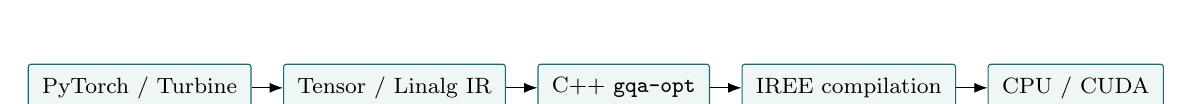
\begin{tikzpicture}[node distance=4mm,box/.style={draw=accent,fill=pale,rounded corners=1pt,minimum height=6mm,font=\footnotesize,inner xsep=5pt},>=Latex]
\node[box](a){PyTorch / Turbine};
\node[box,right=of a](b){Tensor / Linalg IR};
\node[box,right=of b](c){C++ \code{gqa-opt}};
\node[box,right=of c](d){IREE compilation};
\node[box,right=of d](e){CPU / CUDA};
\draw[->](a)--(b);\draw[->](b)--(c);\draw[->](c)--(d);\draw[->](d)--(e);
\end{tikzpicture}
\end{center}
\smallnote{Standalone MLIR 19 driver~\cite{mlir}, with a standard-IR bridge to IREE 3.13/LLVM 24 before dispatch creation. Type, shape, SSA identity, indexing, use and lowering-state guards reject unsupported patterns. No new GPU kernel or complete patched in-tree build.}

\newpage
\section{Evaluation protocol}
\smallnote{Standalone C++ MLIR 19 rewriting precedes IREE 3.13/LLVM 24 compilation (\code{89ece87b8985})~\cite{mlir}. GPU: Tesla T4, driver 580.82.07, FP32, TF32 off. SmolLM2-135M-Instruct~\cite{model}, checkpoint \code{12fd25f77366}: 30 layers, 9Q/3KV heads, width 64. Both IREE variants use O3, both GQA flags, identical split-argmax settings, trig repair and f64-preservation flags. Timing excludes compilation, prefill and upload: resident outputs, context synchronization, randomized order, 31 samples/repetition; median of nine repetition medians (three prompts, three repetitions). Nsight Compute 2025.3.1 app-range counters~\cite{ncu} use prompt 0, three independent processes and three calls/range, separately from timing. All 112 final counter exports were rechecked.}

\section{Winner factoring: pretrained two-candidate step}
{\small
\begin{tabularx}{\linewidth}{@{}r r r r r Y@{}}
\toprule
\textbf{Context} & \textbf{Base ms} & \textbf{Opt. ms} & \textbf{Speedup} & \textbf{Latency lower} & \textbf{Total DRAM change}\\
\midrule
2048 &43.264&31.815&\textbf{1.36$\times$}&\textbf{26.46\%}&$-3.91\%$\\
3072 &63.326&60.386&1.05$\times$&4.64\%&$+1.24\%$\\
4096 &82.409&77.858&1.06$\times$&5.52\%&$-0.27\%$\\
\bottomrule
\end{tabularx}}
\smallnote{This comparison isolates concat winner factoring within the repaired IREE pipeline. All natural and forced-winner cases pass, with exact cache prefixes and unchanged inputs. Worst absolute error: $5.05\!\times\!10^{-5}$ (atol$=5\!\times\!10^{-4}$, rtol$=3\!\times\!10^{-3}$). Ordinary decode has no matches. Writes fall but reads rise: full-model DRAM reduction is inconsistent. At context 2048, kernels increase 987$\to$1047/call and logical memcpy remains 188.8\,MB/call.}

\section{Per-transformation operator results}
\smallnote{Speedup $=$ baseline time / optimized time; below 1 means slower. CPU rows are separate synthetic studies, not full-model gains. Suite figures are geometric means. Earlier T4 projection timings include output downloads; final model timings leave outputs resident. Combined gains are not additive. Full per-case times, variant names and source paths: \code{report/study\_results/}.}
{\small
\begin{tabularx}{\linewidth}{@{}P{40mm}P{29mm}Y@{}}
\toprule
\textbf{Transformation} & \textbf{Measured effect} & \textbf{Workload / attribution}\hfill\cite{project}\\
\midrule
Original GQA head reuse &1.86$\times$ CPU&Default lowering only; no extra gain established over both upstream flags plus fusion.\\
Conditional read forwarding &2.04$\times$ CPU&Cache A1: 187.10$\to$91.74\,$\mu$s; same best-correct baseline.\\
Masked gather forwarding &2.52$\times$ CPU&Same A1: 187.10$\to$74.36\,$\mu$s; alternative to conditional reads.\\
Winner factoring alone &1.38$\times$ CPU&2607.34$\to$1885.37\,$\mu$s; with masked forwarding: 723.42\,$\mu$s, \textbf{3.60$\times$ combined}.\\
Adjacent-update coalescing &0.94--0.96$\times$ alone&4--16-token CPU chains. \textbf{2.17--2.34$\times$ combined} with masked forwarding; merging enables a later match.\\
Snapshot protection / COW &2.58$\times$ combined&109.01$\to$42.27\,$\mu$s CPU: protection \emph{plus} masked forwarding vs fastest correct baseline; not protection alone.\\
Key/value projection placement &3.93$\times$ CPU; 1.20$\times$ T4&16 cases per platform vs strong unabsorbed contractions. One decode ablation: key-only 1.92$\times$, value-only 1.95$\times$.\\
Partial RoPE + projection &11.40$\times$ CPU; 1.50$\times$ T4&Four cases per platform; combined pipeline, no isolated RoPE gain. MLA absorption is prior art.\\
Correct contraction fallback &10.63$\times$ CPU&One wide-head case: 131.11$\to$12.33\,$\mu$s vs correct guarded fused lowering; not a gain from the guard itself.\\
Gather normalization / native guard &Correctness enablers&No independent valid speedup established. Wrong stock outputs are excluded from performance baselines.\\
Stable trig reduction &5/9$\to$9/9 cases pass&Earlier matched-valid-case latency overhead: +0.07\% (A), +0.25\% (B); not a speed optimization.\\
Extra aggressive fusion flag &0.97$\times$ at 2048&Earlier repaired B run: 32.02$\to$33.16\,ms; does not consistently help.\\
\bottomrule
\end{tabularx}}

\section{Forwarding on T4: mechanism and negative control}
{\small
\begin{tabularx}{\linewidth}{@{}Y r r r P{36mm}@{}}
\toprule
\textbf{Track B fixture} & \textbf{Base ms} & \textbf{Opt. ms} & \textbf{Speedup} & \textbf{DRAM MB: base $\to$ opt.}\\
\midrule
Small sparse forks&0.288&0.246&1.17$\times$&5.831$\to$0.128 (97.80\% less)\\
Large sparse forks&1.777&1.230&1.44$\times$&178.897$\to$0.137 (99.92\% less)\\
Dense no-rewrite control&0.545&1.268&\textbf{0.43$\times$}&0.285$\to$0.275 (small / variable)\\
\bottomrule
\end{tabularx}}
\smallnote{Conditional forwarding, separate from the model factoring result. Track A large fixture: 1.14$\times$, 178.228$\to$0.132\,MB in a second T4 session. Synthetic checks use independent FP64 NumPy references (atol$=5\!\times\!10^{-5}$, rtol$=2\!\times\!10^{-3}$). The unexplained no-rewrite regression and uncontrolled clocks limit causal attribution.}

\textbf{Limitations.} One FP32 small model and GPU family; custom one-step branching, not complete serving throughput. Logical tensor elimination, physical allocation, DRAM bytes and latency are distinct claims. Incorrect ownership/numerical cases and irregular masked CUDA compile failures remain recorded. No all-GQA, mixed-precision or global-novelty claim is made.

\clearpage
\renewcommand{\refname}{References and attribution}
\smallnote{\textbf{Prior work.} GQA, MLA absorption and decoupled RoPE have identifiable originating papers below. Read-over-write has classical foundations. For selection factoring, adjacent-update merging and this exact compiler repair, no definitive first paper is established here. Cache-sharing papers are related systems precedents, not attribution for our precise MLIR patterns.}
\vspace{3pt}
\begingroup
\small
\setlength{\parskip}{1pt}
\begin{thebibliography}{99}
\setlength{\itemsep}{3pt}
\bibitem{gqa} J. Ainslie, J. Lee-Thorp, M. de Jong, Y. Zemlyanskiy, F. Lebr\'on and S. Sanghai.
\emph{GQA: Training Generalized Multi-Query Transformer Models from Multi-Head Checkpoints}. EMNLP, 2023, pp. 4895--4901. Originating GQA reference.
\url{https://aclanthology.org/2023.emnlp-main.298/}
\bibitem{mqa} N. Shazeer. \emph{Fast Transformer Decoding: One Write-Head is All You Need}. 2019. Introduces multi-query K/V sharing.
\url{https://arxiv.org/abs/1911.02150}
\bibitem{mccarthy} J. McCarthy. \emph{Towards a Mathematical Science of Computation}. Information Processing'62, 1962, pp. 21--28. Classical functional-array foundation; not a GQA optimization paper.
\url{https://www-formal.stanford.edu/jmc/towards/towards.html}
\bibitem{arrays} C. Tinelli / SMT-LIB. \emph{ArraysEx: Functional Arrays with Extensionality}. Formal select/store read-over-write axioms.
\url{https://smt-lib.org/theories-ArraysEx.shtml}
\bibitem{paged} W. Kwon et al. \emph{Efficient Memory Management for Large Language Model Serving with PagedAttention}. SOSP, 2023. KV sharing and copy-on-write precedent; not our compiler factoring pass.
\url{https://arxiv.org/abs/2309.06180}
\bibitem{forkkv} S. Wang, R. Ren and L. Gui. \emph{ForkKV: Scaling Multi-LoRA Agent Serving via Copy-on-Write Disaggregated KV Cache}. 2026. Related branching-cache system, not the first array-law reference.
\url{https://arxiv.org/abs/2604.06370}
\bibitem{deepseek} DeepSeek-AI et al. \emph{DeepSeek-V2: A Strong, Economical, and Efficient Mixture-of-Experts Language Model}. 2024. Secs.2.1.2--2.1.3 explicitly describe MLA weight absorption and decoupled RoPE.
\url{https://arxiv.org/abs/2405.04434}
\bibitem{rope} J. Su et al. \emph{RoFormer: Enhanced Transformer with Rotary Position Embedding}. First arXiv version, 2021. Originating RoPE reference.
\url{https://arxiv.org/abs/2104.09864}
\bibitem{payne} M. H. Payne and R. N. Hanek. \emph{Radian Reduction for Trigonometric Functions}. ACM SIGNUM Newsletter 18(1), 1983, pp. 19--24. Seminal argument-reduction reference; our bounded f64 scheme is not its full algorithm.
\url{https://doi.org/10.1145/1057600.1057602}
\bibitem{online} M. Milakov and N. Gimelshein. \emph{Online Normalizer Calculation for Softmax}. 2018. Online normalization background.
\url{https://arxiv.org/abs/1805.02867}
\bibitem{flash} T. Dao, D. Y. Fu, S. Ermon, A. Rudra and C. R\'e. \emph{FlashAttention: Fast and Memory-Efficient Exact Attention with IO-Awareness}. NeurIPS, 2022. Fused IO-aware attention background, not implemented anew in this project.
\url{https://arxiv.org/abs/2205.14135}
\bibitem{mlir} C. Lattner et al. \emph{MLIR: A Compiler Infrastructure for the End of Moore's Law}. 2020.
\url{https://arxiv.org/abs/2002.11054}
\bibitem{ireesource} IREE contributors. \emph{GeneralizeLinalgNamedOps; BubbleUpExpandShapes; compilation pipelines}. Source pinned to compiler commit \code{89ece87b89852100c0a4ac3d515e14842d090967}. Implementation evidence for existing transformations, not a GQA-specific paper.
\href{https://github.com/iree-org/iree/tree/89ece87b89852100c0a4ac3d515e14842d090967/compiler/src/iree/compiler}{Pinned IREE compiler source}; paths \code{GlobalOptimization/} and \code{DispatchCreation/}.
\bibitem{model} Hugging Face. \emph{SmolLM2-135M-Instruct model card and checkpoint}. Pinned revision in the evaluation protocol.
\url{https://huggingface.co/HuggingFaceTB/SmolLM2-135M-Instruct}
\bibitem{ncu} NVIDIA. \emph{Nsight Compute Profiling Guide}. Application-range replay, metric coverage and cache/clock controls.
\url{https://docs.nvidia.com/nsight-compute/ProfilingGuide/}
\bibitem{project} CS6886 project. \emph{Attention and KV-cache compiler optimizations: implementation, raw results and reproduction}. Experiment-source snapshot \code{71cc40ae53c5e60f2a690e67ffbc64e85969e64f}.
\url{https://github.com/lazarsalt1441/cs6886_project}
\end{thebibliography}
\endgroup
\end{document}
